
\documentclass{cai}
\usepackage{graphicx}

\usepackage[portuguese]{babel}
\usepackage[latin1]{inputenc}
\usepackage{amsmath}
% \usepackage[utf8]{inputenc}
%\usepackage[T1]{fontenc}

 \volume{32}
 \yyear{2017}
 \page{1001}
% \noversion

%% your definitions
\def\bs#1{{\tt\char`\\#1}}
%%


\begin{document}
\label{firstpage}

\title[How to Write a Paper for CAI]
      {A comparative Analysis of Local \\and Cloud Access Assessment for Multimodal Interactive Application}

\author[I.~Ja\v{s}\v{s}ov\'a, M.~Tak\'a\v{c}]
       {Igor \surname{Falc\~ao}, Carlos \surname{Andr\' e}}

\affiliation{Laboratory of Development of Systems\\
Federal University of Para\\
Av. dos Universit\'arios, s/n\\
68746-630\, Castanhal, Brazil}

\email{igorufpa2013.4@gmail.com, carlosandrekun@gmail.com}


%\author[O.~Authors]
%       {Other \surname{Authors}}
%
%\affiliation{Institute of Other Authors\\
%Adress\\
%City, Country}
%
%\email{other.authors@server.edu}

\noreceived{} \nocommunicated{}

\maketitle

\begin{abstract}
With the recent advances on computing, the multimodal interface concept has gained attention as solution where users can interact more naturally with a computer. This paper demonstrates a case study to evaluate access to local and cloud servers with a multimodal interface, quite usual in handling applications in a Digital TV. The contribution is the multimodal application as well as its validation by means of a case study using Quality of Service (QoS) metrics. Besides, a discussion is followed on the use of local and cloud servers with a focus on costs and computational resources. Results are presented considering both technical and financial feasibility of the proposed architectures.  
\end{abstract}

\begin{keywords}
Cloud Computing, Quality assurance, Software, Multimodal Interface and dynamic applications.
\end{keywords}

\begin{mathclass}
39A60 - 97R50
\end{mathclass}


\section{Introduction}

Cloud computing, an interesting means to offer computing and networking as a service on demand, transforms traditional data canter's into a pool of computing services from which the user chooses the service he/she needs and pays only for whatever service that is used [Meixner, 16]. Cloud computing raises some concerns for business, Internet services or ordinary end users when there is a need to deploy services on the Internet. Therefore, a thorough analysis of costs and aspects of cloud computing, such as networking performance, are of great importance [see Taurion, 2009].

With the growth of the Internet of Things (IoT), a multitude of new devices turn into content and information generators, increasing the need for systems such as cloud computing. Moreover, many of such new devices use new interaction models with users, such as facial expressions, gestures, voice, fingerprint, retina reader, etc. 

In this scenario, development of new applications using only a single option of interaction which may be well accepted by all the users is very unlikely. Thus, research studies become essential and must be conducted in such a way that inputs can be collected with multimodal interfaces, and that the user must be able to choose which interface is more suitable for its use.

The multimodal interaction attracts attention among the Digital Television (DTV) applications, since new devices feature multimodal interaction recognition, making the interaction with the users more intuitive. DTV also appears as a 
new form of educational technology, as pointed out by several researchers because of its different characteristics, such as interactivity, which allows the dynamic use of various media contextually [Santos, 16].

The performance analysis of computing resources is a well known activity. However, rapid development of different technology integration leads to the creation of common criteria for quality of service and metrics for their evaluation. It is known that the qualitative parameters for audio/video content consist of two ways of measurement - objective and subjective [Deksnys, 14].

The financial analysis aims at defining which solution between local or cloud computing resources is more financially interesting. Additionally, an assessment of the financial aspects over time is also performed to define the point in time when both solutions cost the same. The results can be used as a baseline for the deployment of new multimodal applications.

The remaining of this paper is organized as follows: in Sec. 2 the related work of this study is presented. In Sec. 3 the authors detail the application developed for this study. In Sec. 4 presents the network setup used for the performance tests and the description of the proposed architectures. The results are presented in Sec. 5, and the conclusions in Sec. 6.

\section{Related Work}
After a literary review, we did not find specific literatures comparing multimodal applications on cloud and local scenarios. In this way, this section reviews works that present concepts that guide this proposal.

Cloud computing has become a solution to offer flexible and scalable computing infrastructure to many applications. Its many applications and features made it very popular [see Singh et al. 15].

In a cloud computing scenario, services are accessed via the Internet and there is usually a higher latency of communication between service providers and their customers when compared to local access. Such scalable services of cloud computing can be used in research, Digital TV applications and to share resources under a certain workload. Cloud computing can also be used in multimodal interaction applications.

Second [Costa et al. 12], Digital TV offers features ranging from the improvement of image quality to the ability to interact with content. With this new TV modality, the viewer with a possibility to play a more active role, interacting with television programs, which in addition to audio and video. 

The multimodal interaction is well studied in the literature, and it has been applied in many different research subjects. In [Janowski et al. 13] the authors analyze the use of gestures and voice control for different tasks found in a virtual environment (web surfing and object manipulation).

In a new scenario, with the emergence of many data centers around the world, heavy loads of commercial and scientific applications run in the so-called resource management cloud, the cloud becomes efficient, for example, to save energy without compromising system performance. According to Dynamic Data Center (DCD) organization, the energy consumption would increase 19\% from 2012 to 2013 [7]. According to statistics from DCD, the expected power consumption for servers increasing by 19\% in 2013 from the previous year [Alahmadi et al. 14].

On the other hand, local server can partially satisfy the need for rapid multimedia data delivery by providing multiple clients with a shared storage location. All clients from a community are connected to the same Local Area Network. The network bandwidth between the local server and the clients is considered to be adequate with respect to sharing content [see Lee et al. 11].

In practice, this shared processing service poses new challenges to means of interaction with digital contents. Thus, people watching TV are no longer passive and want to actively interact with the content. However, the software required for this interaction is not the main concern of content producers. [Oyarzo et al. 14]

In wireless networks, for instance, the authors in [Fazio et al. 16] present an evaluation study that analyzes the needs of users in terms of Quality of Service (QoS), more specifically for subscribers. There has been an extensive investigation on how to offer and ensure service continuity when users in movement need QoS.

Results from published literature of the field were obtained to ensure that they were within minimum QoS standards, thus, certifying the assurance of the user experience. According to [Ren et al. 14], an efficient level of QoS achieved is extremely necessary to avoid interference and moreover performance must be maintained for the multiuser environment. To the best of our knowledge, this is the first work to assess the performance of QoS metrics and correlate it to the financial aspects, using a multimodal application with shared computing resource. The aforementioned works present only one of the aspects used in this paper.

\section{Semantic based Retrieval using Meta data}
The application was developed in order to offer total freedom of interaction to TVDi users, especially using second screen resources to promote access to simultaneous content to conventional TV programming. 

 The application allows the user to interact with the TV using QR code and second screen, but adds a new layer of interaction to facilitate the transmission.
 
While watching some broadcast on the TV, the user can interact with a second screen in order to access additional content or interact with other users in a social-network-like application, remembering that the list of features of the application is exorcised by [see Tab. 1]. The user can also interact with the TV by using gestures or voice control. 

The second screen content can be accessed through a QR-code showed in the screen while watching a show that has additional interactive content, and in this case the interactive content can be accessed at any time. In the assumed scenario, users can start, resume and finalize their interaction at any time without impacting the content being shown on the TV.

In addition to providing users with experience of interaction with Digital TV device, the developed application was also used as a case study to test architectures that will be evaluated on criteria of performance and operational cost.
\begin{figure}
 \centering
 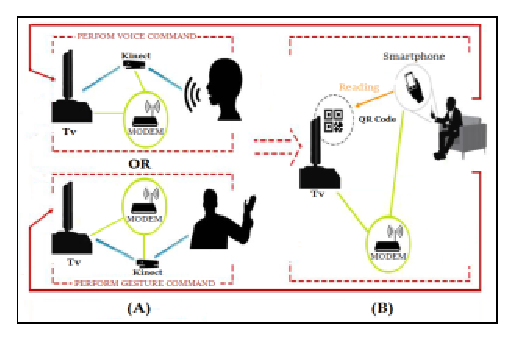
\includegraphics[width=0.4 \linewidth]{images/Picture1.eps}
 \caption{(A) - Gestures and Voice Commands, (B) - QRcode Authentication.}\label{figone}
\end{figure}
[see Fig. 1] shows a scenario where the user watches a TV show and wants further access to interactive content. The equipment is composed by a TV, a Kinect, an Internet modem and a smartphone, all connected to the same WLAN standard IEEE 802.11b on wireless networks with Internet access.

In [see Fig. 1a] the user gives voice commands that are processed by Kinect, and a QR-code is shown on the screen. From that moment, the user can connect the smartphone (as a second screen) to access the additional interactive content, as shown in [see Fig. 1b].

The process just described is similar to the one when the gestures are used in [see Fig. 1a]. It is important to note that at the beginning of the interaction the user is advised about how to use the application and how to give gesture or voice commands.
\section{Document Structure}

A pre-defined \textit{cai} style, the result of a modification of the \textit{article} style, is used for the
papers (\bs{documentstyle\{cai\}}). Document structure is obvious from the source file of this
guide~\cite{cai-style}.

To structure text into sections and subsections, use the commands \bs{section\{\}} and \bs{subsection\{\}}
(or \bs{subsubsection\{\}}).

As a rule, the text to be \textit{highlighted} is italicized \bs{textit\{\dots\}}.


\subsection{Itemizing, Enumerating \dots}

Itemized and numbered lists can be created by help of standard \LaTeX\ environments \textit{itemize} and
\textit{enumerate}. For longer descriptions use lists in the \textit{description} environment.


\subsection{References}

References to literature are listed in the end of the paper text, as shown in this document. To refer to a
concrete literature, use the \bs{cite\{\dots\}} command. As an~example of literature reference, a journal
paper, a book and a conference paper are given~\cite{aklbruda, hintikka, marektruszczinski}.

To refer to a section of the text, use the \bs{label\{\dots\}} and \bs{ref\{\dots\}} commands.

\section{Inserting specials}

\subsection{Tables}

To insert tables, use the \textit{table} environment:

\begin{verbatim}
\begin{table}
 ...
 \caption{Caption for this table}\label{tabone}
\end{table}
\end{verbatim}

To create a body of table, use standard \LaTeX\ methods. We did not create a~body of table in the
\textit{table} environment.

\subsection{Figures}

To insert figures, use the \textit{figure} environment:


%\begin{figure}
 %\centering
 %\includegraphics[width=0.4 \linewidth]{images/}
% \caption{Caption for this figure}\label{figone}
%\end{figure}

To include external figures, Figura \ref{figone} use the \bs{includegraphics\{file.pdf\}} command from the \textit{graphicx}
package. External figures are admissible in the Encapsulated Post\-Script (\texttt{.eps}) or PDF (\texttt{.pdf}) format.

Figures can also be created by help of the techniques available directly in \LaTeX, or in PSTricks.

\subsection{Mathematical Constructions}

Mathematical formulas are enclosed in \$ as the math bracket. To insert equations, use the \$\$\dots\$\$
constructions. To insert numbered equations, or equations to be referred to, use the \textit{equation}
environment.
\begin{verbatim}
\begin{equation}
 ...
 \label{eqno1}
\end{equation}
\end{verbatim}
For multi-line equations, use the \textit{eqnarray} environment:
\begin{verbatim}
\begin{eqnarray[*]}
 var_1  & rel_1  & eq1 \\
 var_2  & rel_2  & eq2 \\
 ...
\end{eqnarray[*]}
\end{verbatim}

\subsection{Lemmas, Proofs\dots}

To write Proofs, use the \textit{proof} environment:

\begin{verbatim}
\begin{proof}
 ...
\end{proof}
\end{verbatim}

If you need further (numbered) environments to express mathematical structure, define them according to the
following example:
\newtheorem{lemma}{Lemma}
\begin{verbatim}
\newtheorem{lemma}{Lemma}
\end{verbatim}

\begin{lemma}[Hopcroft]
This is Lemma\dots
\end{lemma}


\section{Conclusions}

We believe that this short guide will help you to write papers for CAI. In case of any technical problems,
contact us at \texttt{cai@fpv.utc.sk}.

Having finished the paper, send the \TeX\ (\texttt{.tex}) and PDF (\texttt{.pdf}) files to the
Editorial Office. If you insert external figures (\texttt{.eps} or \texttt{.pdf}), include them as well. Use the e-mail
address \texttt{cai.ui@savba.sk}.


\begin{thebibliography}{99}
\bibitem{cai-style}
Ja\v{s}\v{s}ov\'a, I.---Tak\'a\v{c}, M.: CAI Style for Articles. Available on:
\texttt{http://www.cai.sk/style/}, 2003.

\bibitem{cai-web}
CAI web site. Availaible on\hbox{:} \texttt{http://www.cai.sk}.

\bibitem{aklbruda}
Akl, S.~G.---BRUDA, S.~D.: Parallel Real-Time Optimization: Beyond Speedup. Parallel Processing Letters,
Vol.~9, 1999, No.~4, pp.~499--509.

\bibitem{hintikka}
Hintikka, J.: Knowledge and Belief: An Introduction to the Logic of Two Notions. Cornell University Press,
Ithaca, NZ, 1962.

\bibitem{marektruszczinski}
Marek, W.---Truszczinski, M.: Relating Autoepistemic and Dolomit Logic. In: R.~Brachman and H.~Levesque
(Eds.): Principles of Knowledge Representation and Reasoning, Proceedings of the First International
Conference, KR'89, Toronto, May 1989, pp.~276--288.
\end{thebibliography}


\bio{}Ivana,Ja\v{s}\v{s}ov\'a\\ works in the CAI Editorial Office. \dots

\bio{}Marcel,Tak\'a\v{c}\\ works for the CAI Editorial Office. \dots


\label{lastpage}
\bibliography{abbrv}
\bibliography{sigproc2}
\end{document}
